\documentclass[10pt]{article}
\usepackage{fullpage}
\usepackage[utf8]{inputenc}
\usepackage{url}
\usepackage{graphicx}

\input macros

\begin{document}

\noindent TA: Ondřej Čertík\\
web: \url{http://hpfem.math.unr.edu/~ondrej/}\\
class: MATH 181\\
date: January 27, 2009

\section*{Quiz 2 \& 3}

\subsection*{Problem 1}

Sketch the graph of an example of a function $f$ that satisfies all of the
given conditions:
$$\lim_{x\to4^+}f(x)=2\,,\quad
\lim_{x\to4^-}f(x)=1\,,\quad\lim_{x\to1}f(x)=5\,,$$
$$f(4)=2\,,\quad f(1)\ \hbox{is undefined}.$$

\subsection*{Problem 2}

Calculate the following limit:
$$\lim_{h\to0}{(h+3)^3-27\over h}$$

\section*{Solution to Problem 1}

First we draw the conditions given by the limits into a graph:

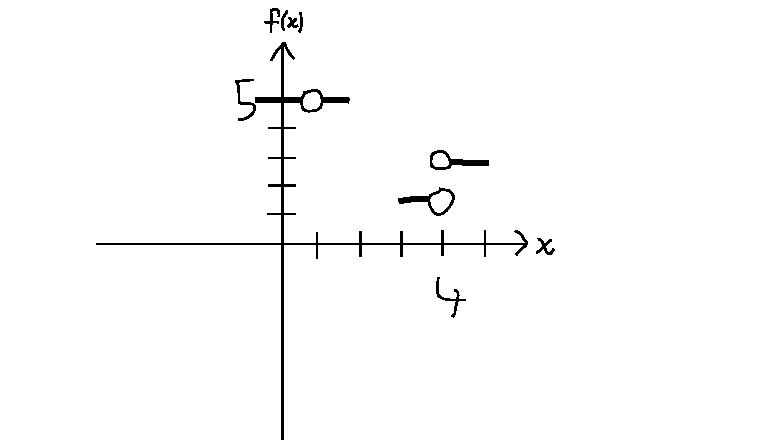
\includegraphics{diag1.pdf}

So far we don't know anything about the function values at the points 1 and 4,
so we just draw empty circles. We however know the behavior of the function in
the neighborhood of the limit (e.g. either from the right or left hand side),
this is denoted by the short graph of the function $f(x)$ around the points.

Next we add in there the function values. $f(4)=2$, so we draw a full circle at
the point 4. $f(1)$ is undefined, so we don't do anything:

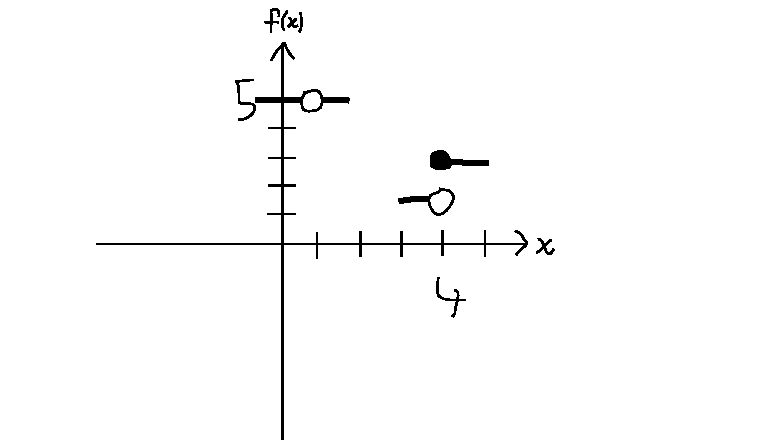
\includegraphics{diag2.pdf}

All the conditions are in the graph and now we are free to finish the plot of
the function $f(x)$ in any way we want, as long as we connect the parts of the
graph already there. One example is here:

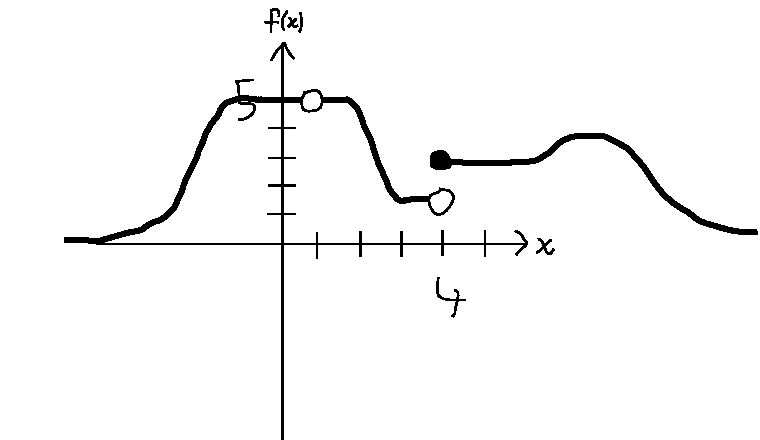
\includegraphics{diag3.pdf}

Another example is:

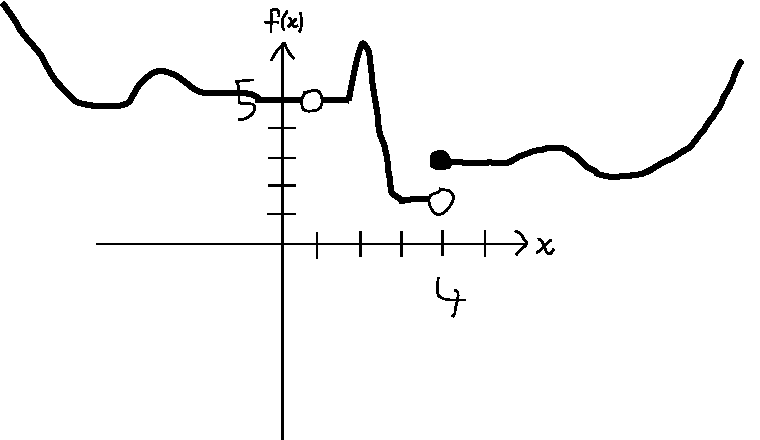
\includegraphics{diag4.pdf}

\subsection*{Grading}

If you got the limits points right, you got $+6$ points, for the function
values $+2$ and for connecting the points correctly $+2$.

\section*{Solution to Problem 2}

We use the formula $(a+b)^3 = a^3+3a^2b+3ab^2+b^3$ to expand the nominator,
then everything cancels out and we are able to calculate the limit:
$$
\lim_{h\to0}{(h+3)^3-27\over h}
=\lim_{h\to0}{h^3+3h^2\cdot3+3h\cdot3^2+3^3-27\over h}
=\lim_{h\to0}{h^3+9h^2+27h+27-27\over h}
=
$$
$$
=\lim_{h\to0}{h^3+9h^2+27h\over h}
=\lim_{h\to0}(h^2+9h+27)
=27
$$

\subsection*{Grading}

You got 2 points if if you got the expression $\lim_{h\to0}{h^3+3h^2\cdot3+3h\cdot3^2+3^3-27\over
h}$ right, another 2 points if you got to the expression
$\lim_{h\to0}{h^3+9h^2+27h+27-27\over h}$, another if you got to the
$\lim_{h\to0}{h^3+9h^2+27h\over h}$, another if you got to the
$\lim_{h\to0}(h^2+9h+27)$ and final 2 points if you got the right answer 27.

\end{document}
